\chapter{Testing}

% Detailed descriptions of every test case are definitely not what is required here. What is important is to show that you adopted a sensible strategy that was, in principle, capable of testing the system adequately even if you did not have the time to test the system fully.

% Have you tested your system on �real users�? For example, if your system is supposed to solve a problem for a business, then it would be appropriate to present your approach to involve the users in the testing process and to record the results that you obtained. Depending on the level of detail, it is likely that you would put any detailed results in an appendix.

% The following sections indicate some areas you might include. Other sections may be more appropriate to your project. 

\section{Overall Approach to Testing}
My approach to testing was using Test Driven Development and refactoring, taking note from XP practices, ensuring that I only developed as much as was required to make tests pass based upon my requriements for eachi part of the applications intended functionality. The aim was to have as many tests automated as possible, as this would allow me to test frequently and reliably and tie into testing everytime I checked into my Git repository with CodeShip's continuous integration of my code. Where automation could not be carried out, I created test files and used a test table to determine whether my application met the requirements I could test against.

%=== Up to here ===

\section{Automated Testing}
\subsection{Unit Tests}
Writing unit tests before writing any functional code to match against was very useful, allowing me to develop code againsts the tests, written one by one, so that I would not develop any more than necessary. This made is so that what was developed fit the requirements, as the tests written before the code were based upon the exact specifications of the requirements. Refactoring the code after each test kept my design evolving and improving maintainability and simplicity to remove duplicate and unnecessary code.

\begin{figure}[H]
\centering
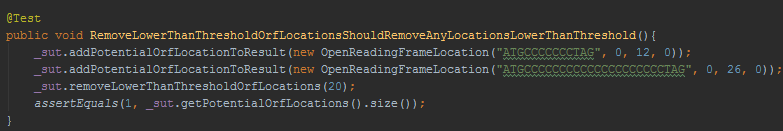
\includegraphics[width=0.9\textwidth]{images/unittestexample}
\caption{An example of a unit test used in my application.}
\end{figure}

Each unit test was made to only carry out one function check at a time, and the naming of each test reflected what the functionality of the system part under test should do. It is for this reason that the item under test is called `sut', system under test, and each test is named with a convention that has a `should' clause in the name, to demonstrated that the function called should produce particular expected results.

\begin{figure}[H]
\centering
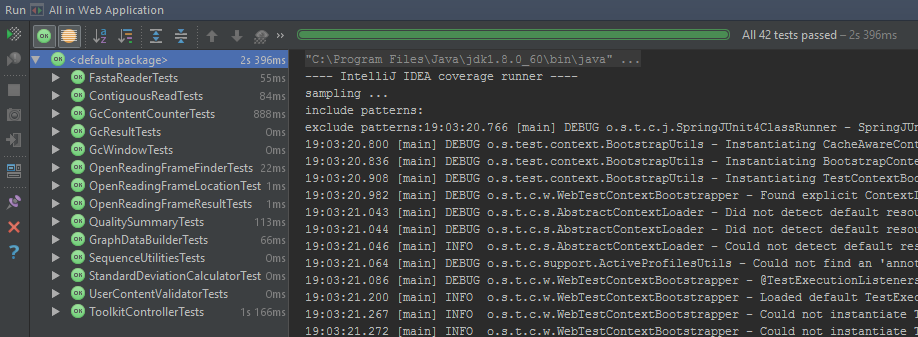
\includegraphics[width=0.9\textwidth]{images/unittestsuccess}
\caption{Results of running the set of unit tests developed for the application.}
\end{figure}

IntelliJ gave  me the tools to run my unit tests with coverage, allowing me to see how much of my code was actually tested against. In the figure below it can be seen that most of my methods were covered. Those methods that were not covered I chose not to test against, as they are mostly setters and getters with no further functionality. In practice, it would perhaps be best to test against these too, in case for some reason the way a value is set or retrieved had to take into account some processing.

\begin{figure}[H]
\centering
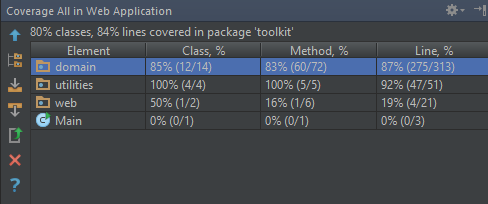
\includegraphics[width=0.9\textwidth]{images/testcoverage1}
\caption{The test coverage of my unit tests over the developed application code.}
\end{figure}

\begin{figure}[H]
\centering
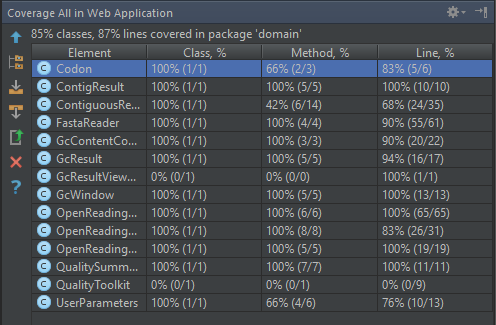
\includegraphics[width=0.9\textwidth]{images/testcoverage2}
\caption{The test coverage of my unit tests over the developed application code, broken down for each class.}
\end{figure}

\subsection{User Interface Testing}
For testing the user interface, I used Chrome's Developer Tools for checking the correct running of the JavaScript, and debugging the code as it ran on loading of the page. I also confirmed that each of my pages loaded and functioned correctly in Google Chrome, Firefox and Microsoft Edge.

\begin{figure}[H]
    \centering
    \begin{subfigure}[b]{0.4\textwidth}
        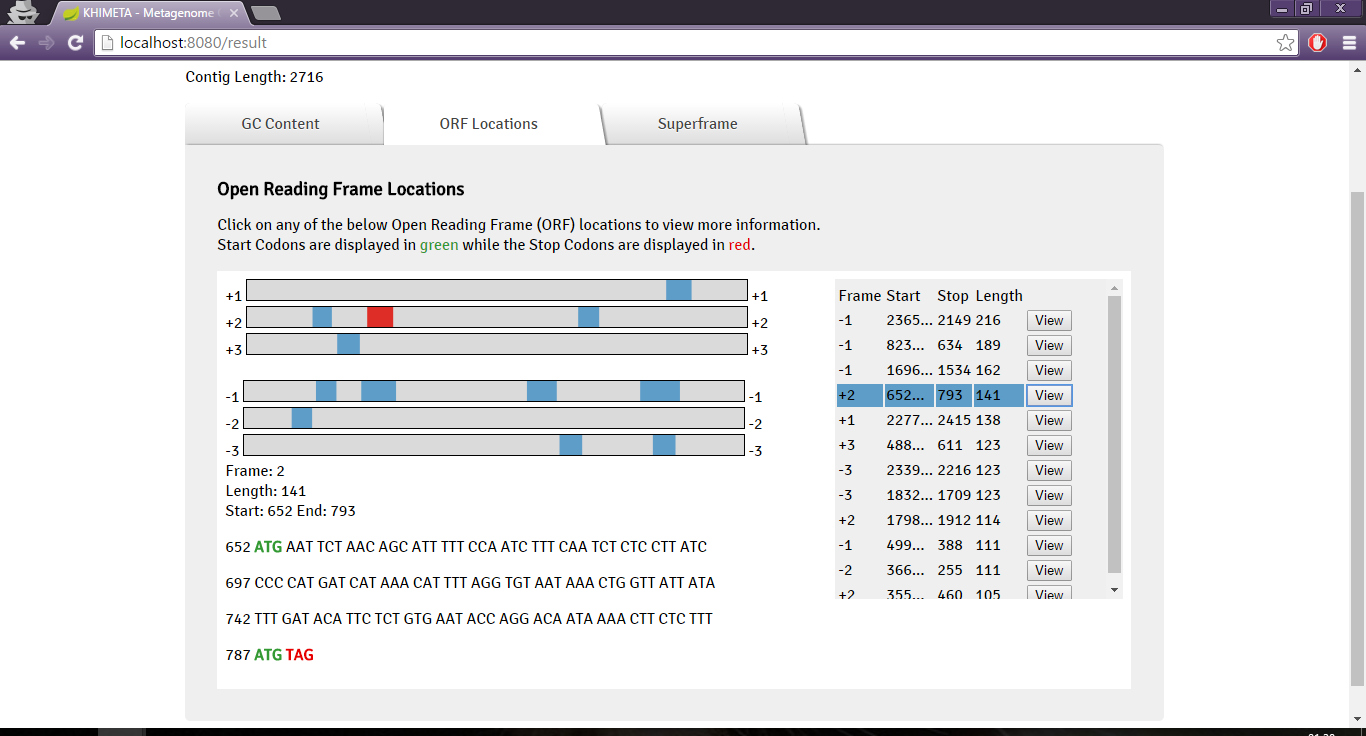
\includegraphics[width=\textwidth]{images/browserchrome}
        \caption{Google Chrome.}
    \end{subfigure}
    ~ %add desired spacing between images, e. g. ~, \quad, \qquad, \hfill etc. 
      %(or a blank line to force the subfigure onto a new line)
    \begin{subfigure}[b]{0.4\textwidth}
        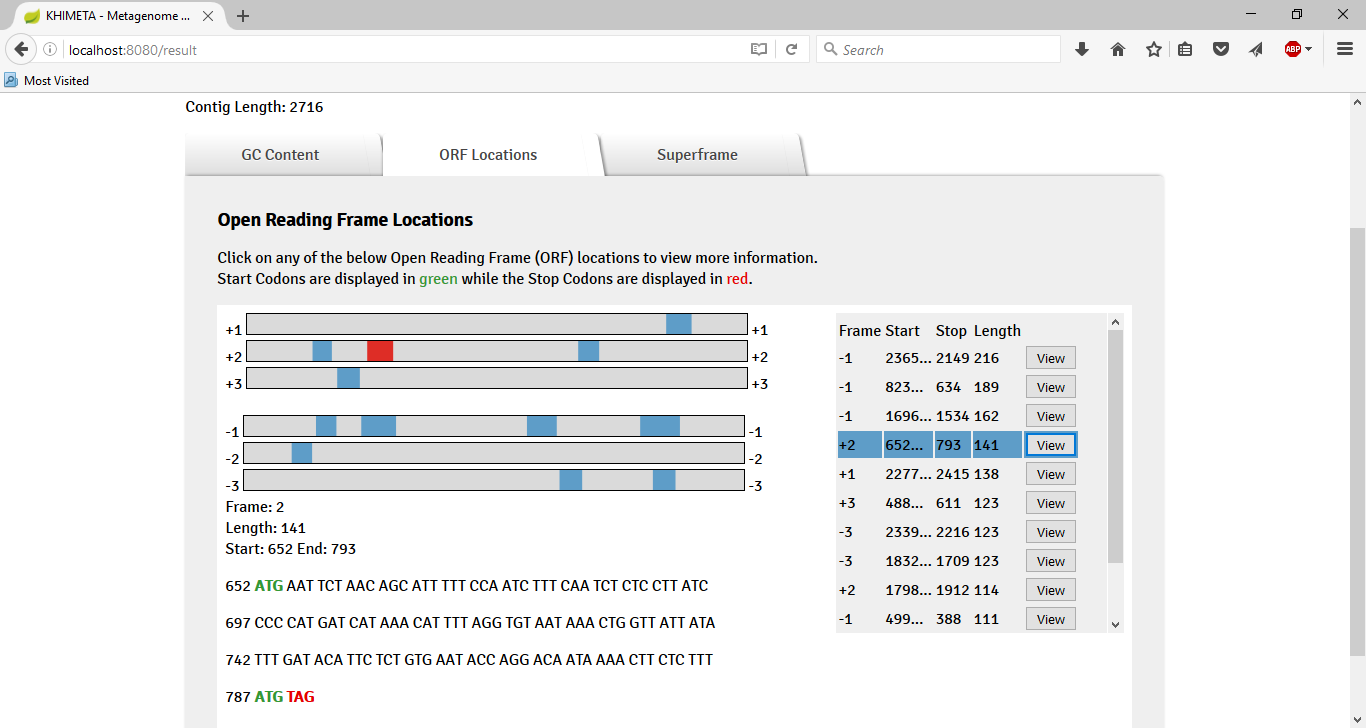
\includegraphics[width=\textwidth]{images/browserffox}
        \caption{Firefox.}
    \end{subfigure}
    ~ %add desired spacing between images, e. g. ~, \quad, \qquad, \hfill etc. 
    %(or a blank line to force the subfigure onto a new line)
    \begin{subfigure}[b]{0.4\textwidth}
        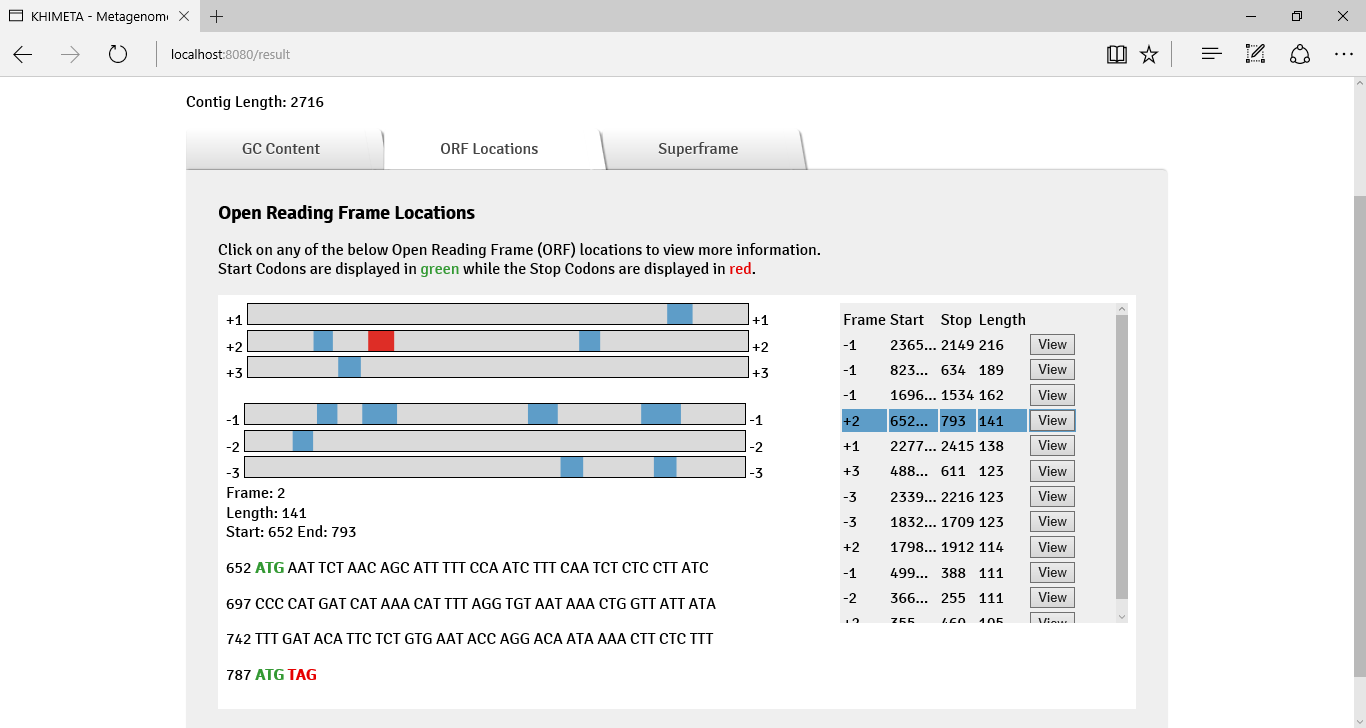
\includegraphics[width=\textwidth]{images/browseredge}
        \caption{Microsoft Edge}
    \end{subfigure}
    \caption{The same page and results from the application shown in different modern browsers.}
\end{figure}

For testing the speed performance of the web pages of the applications loading time, I used YSlow\cite{yslow} which runs a number of checks on the page setup and loading speed to return a report about whether a page loads quickly or slowly, and how it could be improved.

\begin{figure}[H]
\centering
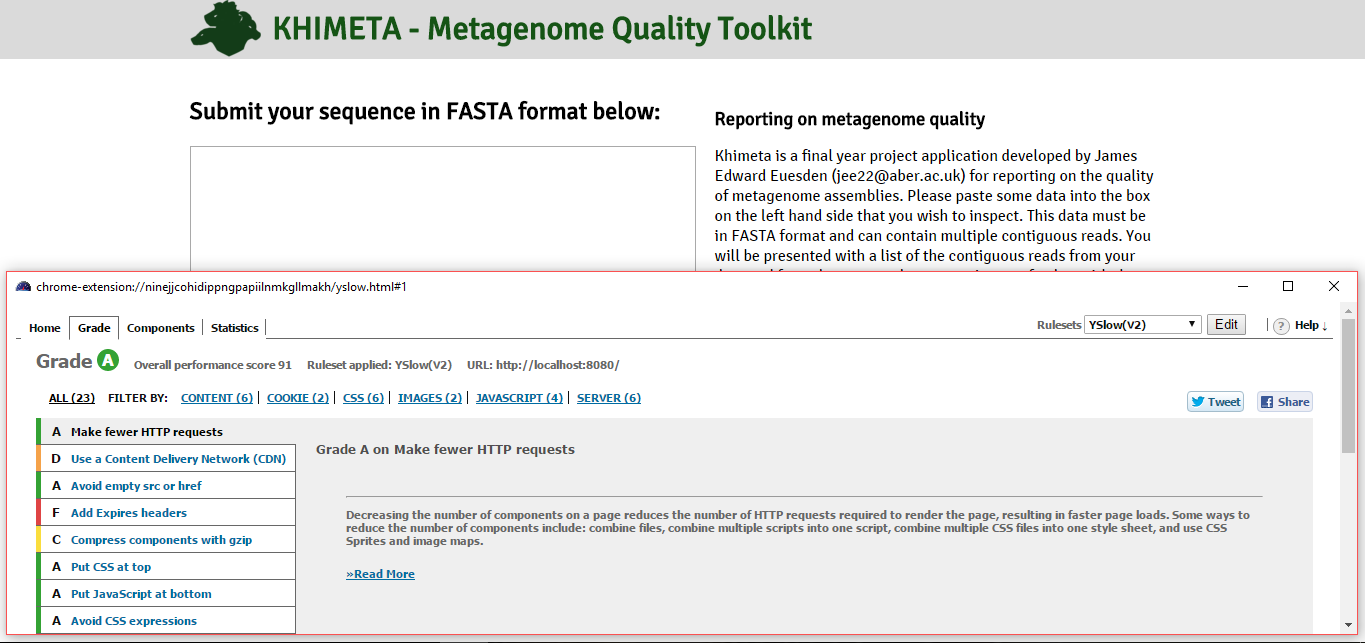
\includegraphics[width=0.8\textwidth]{images/yslowpage1}
\caption{YSlow report after running on the Welcome page.}
\end{figure}

\begin{figure}[H]
\centering
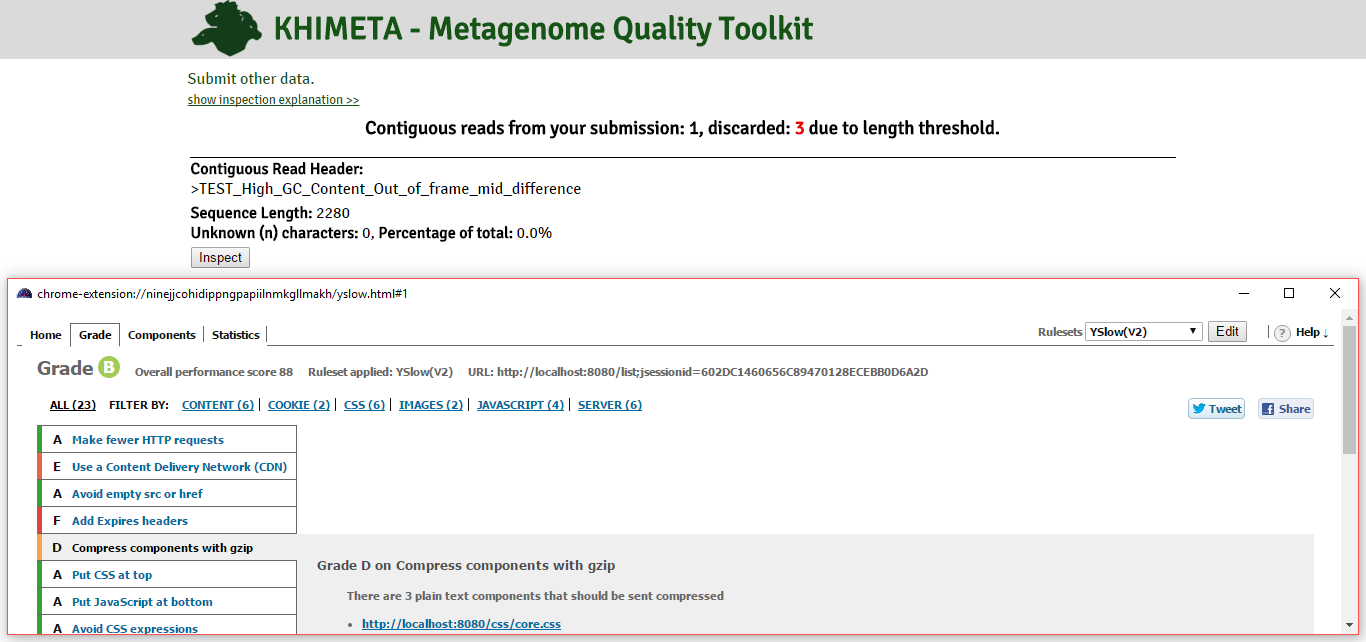
\includegraphics[width=0.8\textwidth]{images/yslowpage2}
\caption{YSlow report after running on the List page.}
\end{figure}

\begin{figure}[H]
\centering
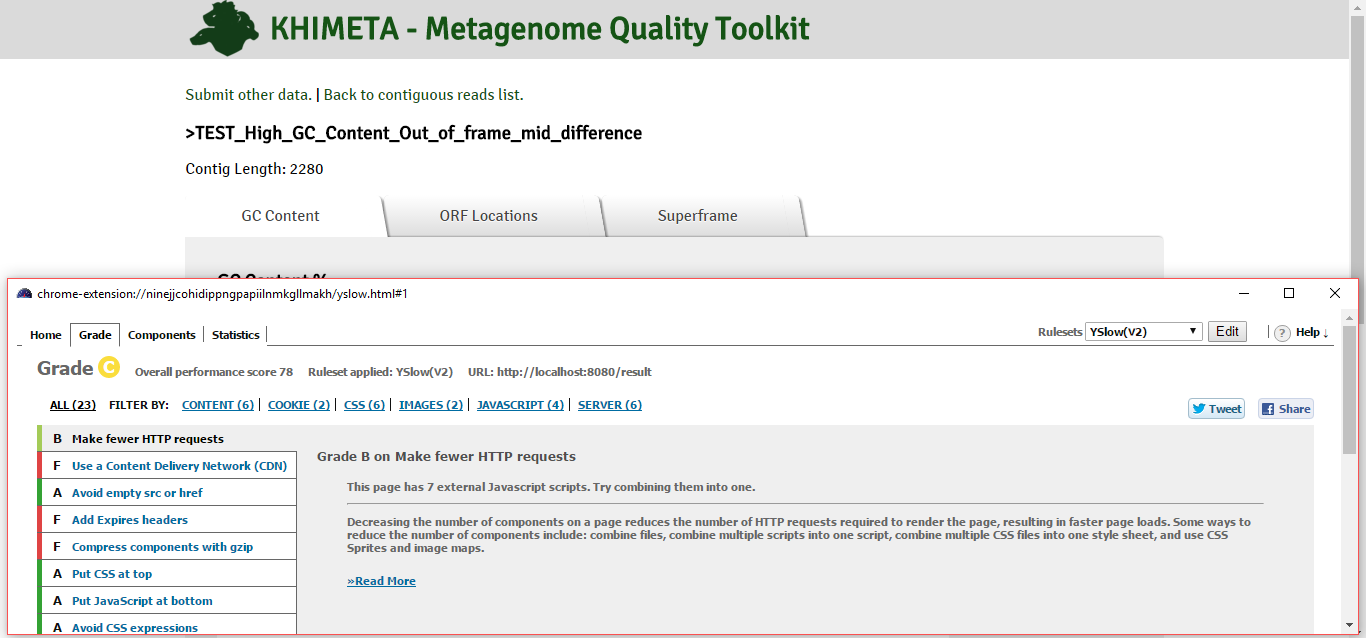
\includegraphics[width=0.8\textwidth]{images/yslowpage3}
\caption{YSlow report after running on the Results page.}
\end{figure}

My results showed me that for the most part there was not much I could do to improve my application outside adding expiry headers to some session variables and implementing a Content Delivery Network (CDN), which was far outisde the scope of the project.

\subsection{Manual Testing}
A number of artificial test files were created in order to be used for testing. Some of these were used in automated tests, such as checking for a files existence and possibility of being read, or throwing exceptions when a test file did not exist while other files were for running manually, either being entirely artificial and checking for individual expected behavours or composed of actual data from multiple species that I manually split and combined together to view the results of. The completely artificial file data is included in the appendices. While the results of the mixed real species data is not included, the results of one very obvious combining of species can be seen in the figure below.

\begin{figure}[H]
\centering
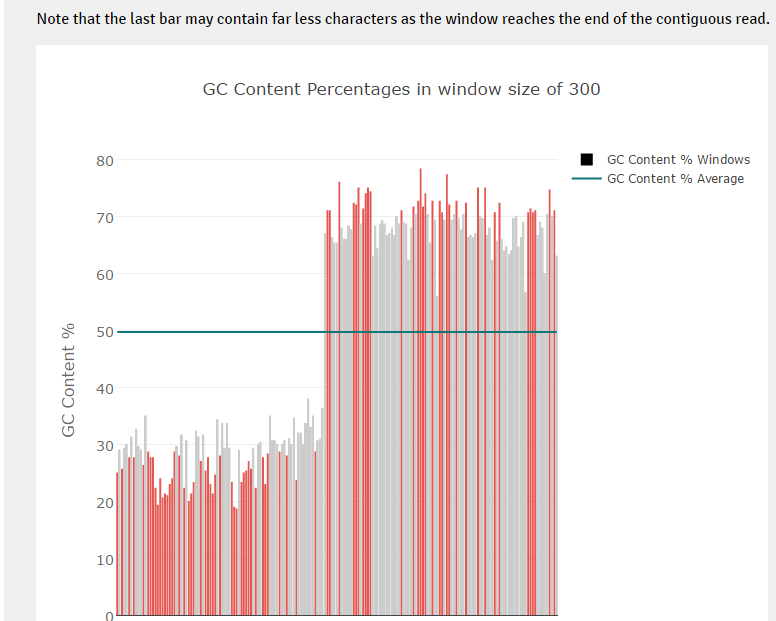
\includegraphics[width=0.7\textwidth]{images/combinedspecies}
\caption{Combining two species contiguous reads together at 50\% of each of the file (first half one species, second half another species), we see a very obvious split in the GC chart.}
\end{figure}

Running this test showed me that it is possible to see where there is a huge change in GC content, but that the threshold won't pick it up because with a case like this, while extremely unlikely to happen where there is a mix of only two species, the threshold only shows those outside of the mean, not drastic changes. It highlights that there is room for improvement with detecting these changes and reporting on them to the user, rather than having them infer it themselves.

\subsubsection{Test Table}
For confirming functional requirements were met and testing things that couldn't be done with automation, I produced a test table with tests matching requirements, expected results and avoiding unwanted results. The tests from the table were carried out by fulfilling the action in the table, and then viewing the results and marking whether the expectations were met or not.

%==== INSERT TEST TABLE HERE ==== 

When it came to running large files, or files with many contigs, I ran a number of my laptop and for the most part it handled them quite well with a few hundred contigs of moderate length, although with contigs in the sizes of a hundred thousand characters and up, the process of reading in the contigs and then processing one starts taking noticably longer. I believe this is a restriction with my own machine, however, as should the JVM be allotted enough memory while the application is hosted on a larger, faster machine it is likely it could perform far better.
